\documentclass[tikz]{standalone}
\usepackage{amsmath,amssymb}
\usepackage{pgfplots,multicol}

\pgfplotsset{compat=1.10}
\usepgfplotslibrary{fillbetween}

\begin{document}



 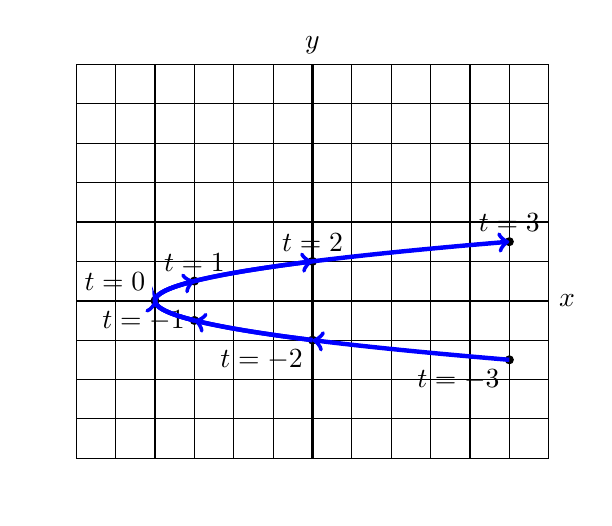
\begin{tikzpicture}[xscale=0.5,yscale=0.5]
        \draw[-,thick] (-6,0) -- (6,0) node[right] {$x$};
         \draw[-,thick] (0,-4) -- (0,6) node[above] {$y$};
\draw[step=1.0,black,thin] (-6,-4) grid (6,6);
%	\foreach \x in {-4,-2,2,4,6}
%	 \draw[-,thick] (\x,0.1) -- (\x,-0.1) node[below] {\x};
%	 
%	 	\foreach \y in {-4,-2,2,4,6}
%	 \draw[-,thick] (0.1,\y) -- (-0.1,\y) node[left] {\y};
	

\draw[fill=black] (5,-3/2) circle (0.1cm) node[below left] {$t=-3$};	
\draw[fill=black] (0,-1) circle (0.1cm) node[below left] {$t=-2$};
\draw[fill=black] (-3,-0.5) circle (0.1cm) node[left] {$t=-1$};
\draw[fill=black] (-4,0) circle (0.1cm) node[above left] {$t=0$};
\draw[fill=black]  (-3,1/2) circle (0.1cm) node[above] {$t=1$};
\draw[fill=black] ( (0,1) circle (0.1cm) node[above] {$t=2$};
\draw[fill=black] (5,1.5) circle (0.1cm) node[above] {$t=3$};

\draw[->,smooth,domain=-3:-2,blue,ultra thick] plot({\x*\x-4},{\x/2});
\draw[->,smooth,domain=-2:-1,blue,ultra thick] plot({\x*\x-4},{\x/2});
\draw[->,smooth,domain=-1:0,blue,ultra thick] plot({\x*\x-4},{\x/2});
\draw[->,smooth,domain=-0:1,blue,ultra thick] plot({\x*\x-4},{\x/2});
\draw[->,smooth,domain=-1:2,blue,ultra thick] plot({\x*\x-4},{\x/2});
\draw[->,smooth,domain=-2:3,blue,ultra thick] plot({\x*\x-4},{\x/2});

\draw[fill=black] (-7,-5) node[above] {};

\end{tikzpicture}


	
\end{document}
